%AUTOR: KAMIL ŁANGOWSKI 
%EMAIL: kamil.langowski@gmail.com
\documentclass[a4paper]{article}

\usepackage{polski}
\usepackage{amsfonts}
\usepackage{listings}
\usepackage{graphicx}
\usepackage{tikz}
\usepackage{geometry}


\lstdefinestyle{mystyle}{
    basicstyle=\ttfamily\footnotesize,
    breakatwhitespace=false,         
    breaklines=true,                 
    captionpos=b,                    
    keepspaces=true,                 
    numbers=left,                    
    numbersep=5pt,                  
    showspaces=false,                
    showstringspaces=false,
    showtabs=false,                  
    tabsize=2
}

\lstset{style=mystyle}
\newtheorem{defi} {Definicja}
\newtheorem{twi}{Twierdzenie}

\title{Algorytm k Najbliższych Sąsiadów}
\author{Kamil Łangowski \\ Wydział Fizyki Technicznej i Matematyki Stosowanej \\ Politechnika Gdańska}
\begin{document}
\maketitle
\newpage
\section{Teoria}
\subsection{Wstęp}
W niniejszej części pracy zajmiemy się omówieniem algorytmu k najbliższych sąsiadów (ang. \textit{k nearest neighbours}), w skrócie zapisujemy kNN. Algorytm kNN jest algorytmem uczenia nadzorowanego, który znajduje zastosowanie zarówno w problemach klasyfikacji (którą omówimy), jak i regresji. Jest jednym z najbardziej podstawowych algorytmów uczenia maszynowego.
\subsection{Zasada działania}
Niech $k$ będzie ustaloną liczbą naturalną, $X$ zbiórem zmiennych objaśniających, $x_j$ będzie obserwacją, którą chcemy zaklasyfikować, a $y\in Y$ jedną z możliwych klas. Klasyfikator wykorzystujący algorytm kNN traktuje każdą obserwację jako punkt w przestrzeni $\mathbb{R}^d$. Wyznacza $k$ najbliższych (w sensie ustalonej metryki) obserwacji do $x_j$, oznaczmy ich zbiór jako $N$. Następnie dokonywana jest estymacja prawdopodobieństwa przynależności obserwacji $x_j$ do klasy $y$ poprzez stosunek liczby  sąsiednich obserwacji klasy $y$ do liczby $k$
\begin{equation}
    P(Y=y|x_j) =\frac{1}{k} \sum\limits_{i \in N}{\delta(y_i, y)},
\end{equation}
gdzie $y_i$ jest etykietą odpowiadającą $i$-tej obserwacji ze zbioru $N$, a funkcja $\delta$, zdefiniowana jako delta Kroneckera\footnote{Leopold Kronecker (1823 -- 1891) -- niemiecki matematyk.} wyraża się wzorem
\begin{equation}
    \delta(y_i,y) = \left\{ \begin{array}{ll}
    1,\quad\textrm{gdy $y_i = y$}\\
    0,\quad\textrm{gdy $y_i \neq y$}
\end{array} \right.
\end{equation}
Następnie algorytm przypisuje obserwację $x_j$ do klasy o dominującym prawdopodobieństwie spośród rozważanych sąsiadów. Na rysunku \ref{r(2.6)}  znajduje się graficzne przedstawienie mechanizmu działania algorytmu kNN. Rozważamy, czy badana obserwacja w tym przypadku  koło będzie należeć do klasy kwadratów czy do klasy trójkątów (zatem jest to klasyfikacja binarna). Jeżeli jako $k$ przyjmiemy 3, wówczas koło zaklasyfikowane zostanie do trójkątów, gdyż obszar wyznaczony przez $k=3$ (okrąg ciągły) zdominowany jest przez obserwacje klasy trójkąt w stosunku 2:1. Natomiast jeżeli ustalimy $k=5$, wtedy koło zaklasyfikowane zostanie jako kwadrat, gdyż w obszarze wyznaczonym przez wybraną liczbę sąsiadów (przerywany okrąg) dominują obserwacje klasy kwadrat w stosunku 3:2.
\begin{figure}[ht]
   \centering
    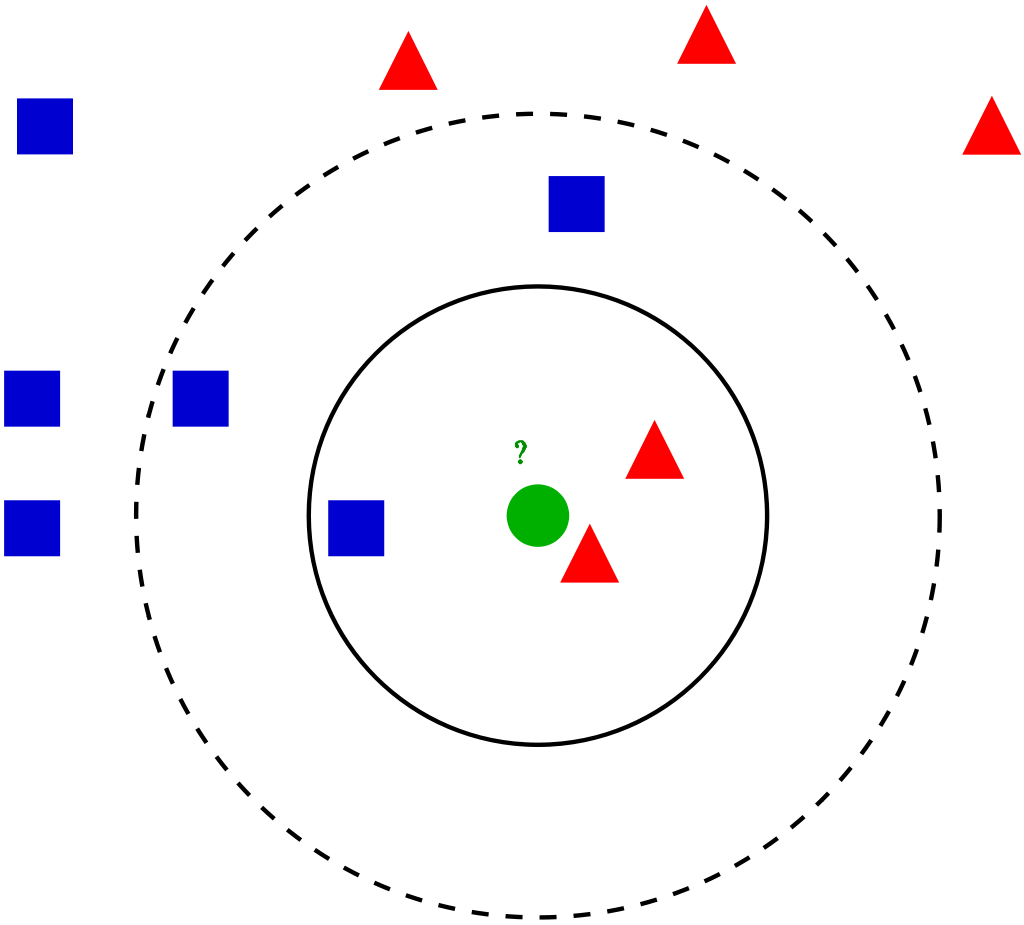
\includegraphics[width=200 pt, height = 180 pt]{knnWIKI.png}
    \caption{Ilustracja działania algorytmu kNN. Źródło: wikipedia -- k-nearest neighbors algorithm.}
    \label{r(2.6)}
\end{figure}
\newpage
\subsection{Pojęcie odległości}
W metodach wykorzystujących algorytm kNN bardzo istotny jest wybór odpowiedniej odległości, którą niekiedy nazywamy miarą niepodobieństwa (gdyż im bardziej zwiększymy odległość pomiędzy dwoma obiektami, tym bardziej są one do siebie niepodobne).
\begin{defi}[Miara niepodobieństwa]
Funkcję $d: \mathbb{R} \times \mathbb{R} \to \mathbb{R}$ nazywamy miarą niepodobieństwa jeżeli:
\begin{enumerate}
    \item $\forall_{x,y\in\mathbb{R}}\quad d(x,y) \geq 0$.
    \item $\forall_{x,y\in\mathbb{R}}\quad d(x,y) = 0 \iff x = y$.
    \item $\forall_{x,y\in\mathbb{R}}\quad d(x,y) = d(y,x)$.
\end{enumerate}
\end{defi}
Tak zdefiniowaną funkcję nazywamy też semi-metryką. Zwróćmy uwagę, że nie jest koniecznym, by funkcja $d$ spełniała warunek trójkąta dla metryk, jako że interesują nas jedynie obserwacje oddalone bezpośrednio od obserwacji badanej. Pomimo tego, funkcja $d$ często spełnia wszystkie aksjomaty metryki. W zależności od charakteru badanej obserwacji wykorzystujemy inne miary niepodobieństwa.  Metryki, które najczęściej wykorzystuje się w algorytmie kNN to m.in. metryka euklidesowa, metryka Mahalanobisa\footnote{Prasanta Chandra Mahalanobis (1893 -- 1972) -- indyjski statystyk.}, metryka Minkowskiego\footnote{Hermann Minkowski (1864--1909) -- niemiecki matematyk i fizyk.}.
\subsection{Wybór k}
Kolejną bardzo istotną kwestią dla algorytmu kNN jest wybór odpowiedniej liczby $k$. Jeżeli $k$ zostanie dobrane jako zbyt duże, może to skutkować niedokładnością predykcji. Z kolei dla małych wartości parametru $k$ predykcja może okazać się zbyt zmienna. Nie ma ściśle określonych metod, które pozwoliłyby ustalić najlepszą wartość $k$. Jednym ze sposobów na wybór $k$ może być stworzenie wykresu zależności niedokładności modelu (stosunek zaklasyfikowanych obserwacji danej klasy do wszystkich obserwacji danej klasy) od liczby $k$, a następnie ustalenie takiego $k$, dla którego niedokładność jest najmniejsza.

\newpage
\section{Przykład}
\subsection{Opis zbioru}
W przykładzie przedstawiającym wykorzystanie algorytmu kNN posłużymy się jednym z najbardziej znanych zbiorów danych w dziedzinie uczenia maszynowego, jest to zbiór \textit{iris}. Zbiór został udostępniony po raz pierwszy w roku 1936. Zawiera informacje na temat trzech gatunków kwiatu irysa: \textit{setosa}, \textit{versicolor}, \textit{virginica}. Każdy z kwiatów opisują 4 atrybuty dotyczące jego wymiarów.
\subsection{Cel}
Naszym celem będzie predykcja gatunku kwiatu irysa na podstawie jego wymiarów.
\subsection{Kod programu}
Importujemy niezbędne pakiety:
\begin{lstlisting}[language=R, frame =single]
library(BBmisc)
library(caret)
library(OneR)
\end{lstlisting}
Pakiet \textit{BBmisc} zawiera funkcję \textit{normalize} służącą do normalizacji danych, którą posłużymy się w dalszej części przykładu. Wyświetlmy więcej informacji na temat zbioru \textit{iris}:
\begin{lstlisting}[language=R, frame=single]
dane <- iris
str(dane)
summary(dane)
\end{lstlisting}
\begin{lstlisting}[language=R, frame=single]
'data.frame':	150 obs. of  5 variables:
 $ Sepal.Length: num  5.1 4.9 4.7 4.6 5 5.4 4.6 5 4.4 4.9 ...
 $ Sepal.Width : num  3.5 3 3.2 3.1 3.6 3.9 3.4 3.4 2.9 3.1 ...
 $ Petal.Length: num  1.4 1.4 1.3 1.5 1.4 1.7 1.4 1.5 1.4 1.5 ...
 $ Petal.Width : num  0.2 0.2 0.2 0.2 0.2 0.4 0.3 0.2 0.2 0.1 ...
 $ Species     : Factor w/ 3 levels "setosa","versicolor",..: 1 1 1 1 1 1 1 1 1 1 ...
 
   Sepal.Length    Sepal.Width     Petal.Length    Petal.Width          Species  
 Min.   :4.300   Min.   :2.000   Min.   :1.000   Min.   :0.100   setosa    :50  
 1st Qu.:5.100   1st Qu.:2.800   1st Qu.:1.600   1st Qu.:0.300   versicolor:50  
 Median :5.800   Median :3.000   Median :4.350   Median :1.300   virginica :50  
 Mean   :5.843   Mean   :3.057   Mean   :3.758   Mean   :1.199                  
 3rd Qu.:6.400   3rd Qu.:3.300   3rd Qu.:5.100   3rd Qu.:1.800                  
 Max.   :7.900   Max.   :4.400   Max.   :6.900   Max.   :2.500 
\end{lstlisting}
Zbiór zawiera 150 obserwacji opisanych przez 5 atrybutów. Są to kolejno:
\begin{itemize}
    \item \textit{Sepal.Length} – długość listka kielicha kwiatowego (zmienna numeryczna),
    \item \textit{Sepal.Width} – szerokość listka kielicha kwiatowego (zmienna numeryczna),
    \item \textit{Petal.Length } – długość płatka kwiatu (zmienna numeryczna),
    \item \textit{Petal.Width } – szerokość płatka kwiatu (zmienna numeryczna),
    \item \textit{Species} -- gatunek kwiatu (zmienna kategoryczna). Jest to nasza zmienna celu.
\end{itemize}
Wszystkie atrybuty wyrażone są w centymetrach, zatem przed zbudowaniem modelu konieczna  będzie normalizacja danych. Zauważmy w kolumnie \textit{Species}, że przykładów każdego gatunku kwiatu jest dokładnie po 50. Sprawdźmy jak wyglądają zależności długość listka kielicha kwiatowego od szerokość listka kielicha kwiatowego dla różnych gatunków:
\begin{lstlisting}[language=R,frame=single]
ggplot(data = iris, aes(x = Sepal.Length, y = Sepal.Width, col = Species)) +
  geom_point()
\end{lstlisting}
\begin{figure}[ht]
    \centering
    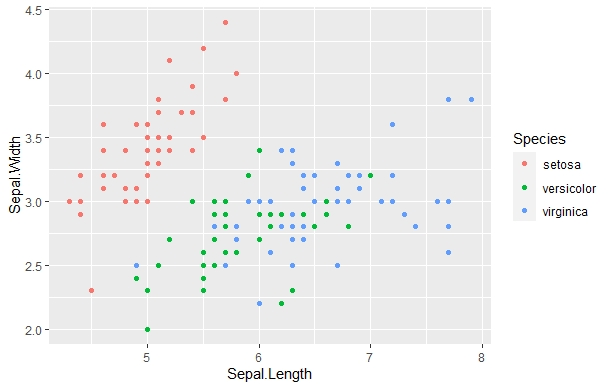
\includegraphics[width = 300 pt]{Sepal_zaleznosc.jpeg}
    \caption{Zależność wymiarów listka kielicha kwiatowego.}
\end{figure}
Na podstawie wykresu niełatwo jednoznacznie określić wyraźne rozróżnienie dla kwiatów z gatunków \textit{versicolor} i \textit{virginica}. Jednakże w przypadku kwiatów \textit{setosa} obserwujemy wyraźne rozgraniczenie dla obserwacji tego gatunku od pozostałych. \newpage
Analogicznie sprawdźmy zależność dla wymiarów płatka kwiatu
\begin{lstlisting}[language=R,frame=single]
ggplot(data = iris, aes(x = Petal.Length, y = Petal.Width, col = Species)) +
  geom_point()
\end{lstlisting}
\begin{figure}[ht]
    \centering
   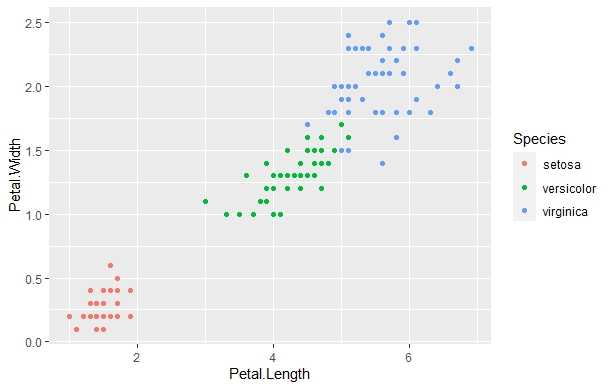
\includegraphics[width = 300 pt]{Petal_zaleznosc.jpeg}
    \caption{Zależność wymiarów płatka kwiatu.}
\end{figure}
W przypadku wymiarów płatka kwiatu z mniejszą trudnością możemy wyróżnić różnice pomiędzy danymi gatunkami, zwłaszcza dla gatunku \textit{setosa}. W następnym kroku dokonamy normalizacji danych wykorzystując do tego zadania wspomnianą wcześniej funkcję \textit{normalize}:
\begin{lstlisting}[language=R,frame=single]
dane_norm <- normalize(dane, method = "range", range = c(0,1))
\end{lstlisting}\newpage
W celu porównania wyświetlmy 6 pierwszych wierszy danych przed i po normalizacji:
\begin{lstlisting}[language=R,frame=single]
  Sepal.Length Sepal.Width Petal.Length Petal.Width Species
1          5.1         3.5          1.4         0.2  setosa
2          4.9         3.0          1.4         0.2  setosa
3          4.7         3.2          1.3         0.2  setosa
4          4.6         3.1          1.5         0.2  setosa
5          5.0         3.6          1.4         0.2  setosa
6          5.4         3.9          1.7         0.4  setosa

  Sepal.Length Sepal.Width Petal.Length Petal.Width Species
1   0.22222222   0.6250000   0.06779661  0.04166667  setosa
2   0.16666667   0.4166667   0.06779661  0.04166667  setosa
3   0.11111111   0.5000000   0.05084746  0.04166667  setosa
4   0.08333333   0.4583333   0.08474576  0.04166667  setosa
5   0.19444444   0.6666667   0.06779661  0.04166667  setosa
6   0.30555556   0.7916667   0.11864407  0.12500000  setosa
\end{lstlisting}

Dokonujemy podziału na zbiór treningowy ($75\%$ zbioru) i zbiór testowy ($25\%$ zbioru):
\begin{lstlisting}[language=R,frame=single]
podzial <- createDataPartition(dane_norm$Species, p=0.75, list=FALSE)
trening <- dane_norm[podzial,]
test <- dane_norm[-podzial,]
\end{lstlisting}
\indent Wykorzystując funkcję \textit{train} z pakietu \textit{cran} tworzymy model oparty na algorytmie kNN:
\begin{lstlisting}[language=R,frame=single]
model <- train(trening[, 1:4], trening[, 5],   method = 'knn')
\end{lstlisting}
Zwróćmy uwagę, że funkcja \textit{train} nie wymaga podawania parametru $k$, gdyż sama dokonuje oceny, jaki wybór $k$ będzie miał największą dokładność. Miarą niepodobieństwa, dla stworzonego modelu jest metryka Minkowskiego. Wyświetlmy więcej informacji na temat modelu:
\begin{lstlisting}[language=R,frame=single]
model
\end{lstlisting}
\begin{lstlisting}[language=R,frame=single]
k-Nearest Neighbors 

114 samples
  4 predictor
  3 classes: 'setosa', 'versicolor', 'virginica' 

No pre-processing
Resampling: Bootstrapped (25 reps) 
Summary of sample sizes: 114, 114, 114, 114, 114, 114, ... 
Resampling results across tuning parameters:

  k  Accuracy   Kappa    
  5  0.9538182  0.9300072
  7  0.9519364  0.9270353
  9  0.9548180  0.9314652

Accuracy was used to select the optimal model using the largest value.
The final value used for the model was k = 9.
\end{lstlisting}
Według funkcji \textit{train} najlepszym wyborem jest przyjęcie $k=9$, dla którego uzyskano dokładność $95.48\%$.\newpage
Dokonujemy predykcji i wyświetlamy podsumowanie modelu:
\begin{lstlisting}[language=R,frame=single]
predykcja <- predict.train(object = model, test[,1:4])

eval_model(test$Species, predykcja)
\end{lstlisting}
\begin{lstlisting}[language=R,frame=single]
Confusion matrix (absolute):
            Actual
Prediction   setosa versicolor virginica Sum
  setosa         12          0         0  12
  versicolor      0         11         1  12
  virginica       0          0        12  12
  Sum            12         11        13  36

Confusion matrix (relative):
            Actual
Prediction   setosa versicolor virginica  Sum
  setosa       0.33       0.00      0.00 0.33
  versicolor   0.00       0.31      0.03 0.33
  virginica    0.00       0.00      0.33 0.33
  Sum          0.33       0.31      0.36 1.00

Accuracy:
0.9722 (35/36)

Error rate:
0.0278 (1/36)

Error rate reduction (vs. base rate):
0.9565 (p-value = 7.69e-15)
\end{lstlisting}
Nasz model prawidłowo przewidział gatunek kwiatu 35 razy z 36 przypadków, oznacza to, że dokładność modelu wynosi $97.22\%$. Jedna pomyłka algorytmu kNN dotyczyła klasyfikacji kwiatu gatunku \textit{virginica} jako gatunku \textit{versicolor}. Zwróćmy uwagę, że są to gatunki, dla których rozdział obserwacji nie był tak wyraźny jak w przypadku kwiatów gatunku \textit{setosa}.


\end{document}
